\subsection{The Transaction Optimization Problem}\label{sec:tx-opt-problem}

Using the above ideas, we now formally define the transaction optimization
problem as a typical \emph{optimization problem}, assuming a set of available
input selection algorithms $\{Sel_1, Sel_2, \dots, Sel_l\}$.

\begin{definition}\label{def:tx-optimization-problem}
    Given $N$ payments between $M$ parties $\party_1, \party_2, \dots, \party_M$ and a
    search space $\mathcal{S}$ of \emph{equivalent} (cf.
    Definition~\ref{def:equiv_total_orders_of_txs}), ordered lists of
    transaction plans that execute the $N$ payments, called \emph{candidate
    solutions}, find the candidate $\tau \in \mathcal{S}$, such that
    $eval(\tau) \leq eval(\rho)$, for all $\rho \in \mathcal{S}$.
    Specifically:
    \begin{enumerate}
        \item A candidate $\rho \in \mathcal{S}$ is an ordered list of
            transaction plans\footnote{We assume that transactions are
            non-correlated (cf. Definition~\ref{def:correlated_tx}) and that all
            orderings are equivalent (cf.
            Definition~\ref{def:equiv_total_orders_of_txs}).} $||T_1||
            \rightarrow
            ||T_2|| \rightarrow \dots \rightarrow ||T_k||$, where the
            transaction plan of
            a transaction $T_x$ is the pair:
            $||T_x|| \defn$ (Logical Expression, Input Selection Algorithm).

        \item The search space $\mathcal{S}$ is defined by all candidates
        $||T_1||
            \rightarrow ||T_2|| \rightarrow \dots \rightarrow ||T_k||$, where,
            for each
            transaction $T_i$, an input selection algorithm from
            $\{Sel_1, Sel_2, \dots, Sel_l\}$ is chosen and, possibly, the 2-for-1 logical
            transformation (cf.  Definition~\ref{def:2-for-1}) is applied.

        \item $eval$ evaluates the cost of every candidate $\rho \in
            \mathcal{S}$ (cf. Definition~\ref{def:tx-cost}) as follows:
            \begin{align*}
                eval : [Transaction] \rightarrow LedgerState \rightarrow Cost,
                \\
                eval([T_1, T_2, \dots, T_k], \ledgerState_{init}) = \\
                cost((txRun(T_k).\ \dots\ .txRun(T_2).txRun(T_1))(\ledgerState_{init})) - cost(\ledgerState_{init})\\
            \end{align*}
            where $cost(S) = |S|$ is the size of a ledger state (cf.
            Definition~\ref{def:lstate}) and the functions $(txRun(T_k).\ \dots\
            .txRun(T_2).txRun(T_1))(\ledgerState_{init})$ output the final
            state after the list of ordered transactions is executed on the
            initial state $\ledgerState_{init}$, according to each individual
            transaction plan $||T_i||$.
    \end{enumerate}
\end{definition}

\paragraph{Solving the Transaction Optimization Problem}

We now present a 3-step, dynamic programming algorithm, which solves the
transaction optimization problem via an exhaustive search and
dynamically pruning candidate solutions:
\begin{enumerate}
    \item Create $N$ transactions $T_{ij}$, $i,j \in [1,M]$,
        corresponding to the payments ($\party_i \xrightarrow[]{V_{ij}} \party_j$),
        as follows:
        \begin{equation*}
            T_{ij} = (\sigma_{\party_i, V_{ij}}(\ledgerState_{init})) \infixOperator (\pi_{\party_j,V{ij}}(\ledgerState_{init}))
        \end{equation*}
        where $V_{ij}$ is the amount to be paid from $\party_i$ to $\party_j$.
        For each $T_{ij}$, find the input selection algorithm in
        $\{Sel_1, Sel_2, \dots, Sel_l\}$ that minimizes $eval(T_{ij},
        \ledgerState_{init})$. Then, enforce the \emph{heuristic rule} to
        create a \emph{single} output per recipient address for each
        transaction.
        At the end of this step, the algorithm outputs $N$ transaction plans,
        \ie $N$ pairs of transaction's $T_{ij}$ logical expression and the
        chosen
        input selection algorithm:
        \begin{equation*}
            ||T_{ij}|| = ((\sigma_{\party_i, V_{ij}}(\ledgerState_{init})) \infixOperator (\pi_{\party_j,V{ij}}(\ledgerState_{init})),\; Sel_s)
        \end{equation*}

    \item On each transaction plan output of Step 1, perform a 2-for-1
        transformation (cf. Definition~\ref{def:2-for-1}). This step produces a
        transformed transaction as
        depicted in Figure~\ref{fig:search_alg_2-for-1}, based on an amount
        $p\times V_{ij}$, where $p$ is a
        configuration parameter of the algorithm, typically in the range $0 < p
        \leq 1$.
        Then, for each of the two transactions that comprise the 2-for-1
        transformation, choose the input selection algorithm that minimizes the
        $eval$ function and enforce the heuristic rule of a \emph{single}
        output per recipient address.  Finally, accept the 2-for-1 transformed
        transaction only if its cost (given by $eval$) is smaller than the
        non-transformed transaction.

        \begin{figure}[h!] %[H]
                \centering
                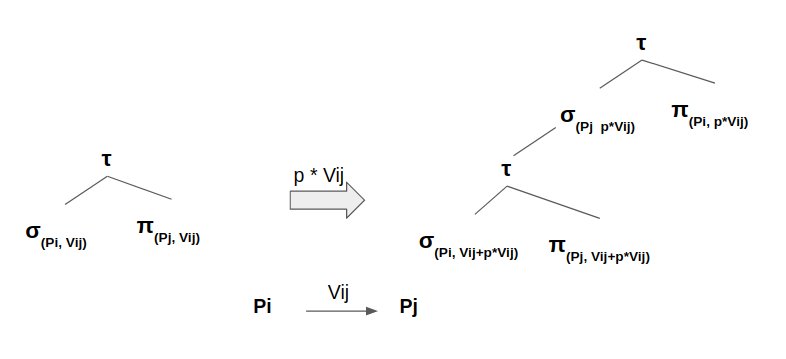
\includegraphics[width=0.8\columnwidth,keepaspectratio]{figures/utxo_growth/search_alg_2-for-1.png}
                \caption{Applying the 2-for-1 transformation to each separate
                transaction.}
                \label{fig:search_alg_2-for-1}
        \end{figure}

        At the end of this step, the algorithm outputs $k$ transaction plans,
        $k \geq N$, comprising of the 2-for-1 transformed and the
        non-transformed transactions, along with their input selection
        algorithms. Importantly, at this point, the algorithm has an optimal
        plan for each \emph{individual} payment ($\party_i
        \xrightarrow[]{V_{ij}} \party_j$), based on an exhaustive search of
        solutions and cost-driven choices.

    \item In this step, the algorithm finds the optimal total order to
        execute the $k$ transactions produced on Step 2. Since there exist $k!$
        permutations, the search space is pruned using the
        \emph{Last-Payer heuristic rule} (cf.
        Section~\ref{sec:tx_optimization_techniques}).
        At the end of this step, the algorithm outputs a totally ordered set of
        transaction plans that solve the optimization problem, \ie executes the
        $N$ payments with a minimum state ledger cost.
\end{enumerate}

Our algorithm's \emph{asymptotic time complexity} depends on its slowest
element.  For simplicity, we assume that applying a transaction on a ledger
state requires constant time. Therefore, in Step 1, creating each of the $N$
transactions is $O(1)$. However, each of the $l$ input selection algorithms may
have different complexity when parsing the $n$ UTxO inputs. For
example,~\cite{karakostas2021efficient} shows that to minimize ``change'', \ie
to find inputs that exactly match the payment's output, requires solving a
Knapsack problem, \ie $O(2^n)$, but is not necessarily state efficient;
instead, the paper proposes an input selection algorithm with complexity $O(n
\log n)$. Step 2 has the same asymptotic complexity as Step 1, as performing
the 2-for-1 transformation requires $O(1)$, as does the application of
heuristics, while choosing an input selection algorithm is the same as in Step
1. Finally, Step 3 requires $O(N!)$, in the corner case when the heuristics do
not prune the search space at all.

On the whole, assuming the complexity of the least efficient input selection
algorithm is $O(\lambda(n)$, our algorithms complexity is $O(\lambda(n) + N!)$,
where $n$ are the available inputs and $N$ is the number of payments.
Theoretically speaking, this is a rather inefficient solution. In practice
though, the wallets of regular users do not control many UTxOs, so $n$ is
expectedly low. The same holds for $N$, as regular users are not expected to
perform complex payments towards multiple third parties.  Nonetheless,
optimizing the employed modules, \eg designing more efficient input selection
algorithms and heuristics, offers an interesting path for future research.

Regarding \emph{optimality}, the transaction plans produced in Step 2 are
optimal \wrt executing the individual transactions, since the algorithm
performs an exhaustive search for the minimum-cost solution. In Step 3, the
algorithm is based on a heuristic rule (Last-Payer) to search for the optimal
total order in a pruned (and thus manageable) space.  Future work will evaluate
the efficiency of this heuristic rule, \ie how well it approximates the optimal
solution, and explore further rules for achieving optimality.
